\documentclass[nocrop, noinfo]{bioinfo}
\usepackage{listings}
\usepackage{graphicx}
\usepackage{xcolor}
%\usepackage{xurl}
\let\href\undefined
\usepackage[
	colorlinks = true,
	linkcolor = blue,
	urlcolor  = blue,
	citecolor = brown,
	anchorcolor = blue
	]{hyperref}

\copyrightyear{2021} \pubyear{2021}

\lstset{frame=tb, language=bash}

\access{}%Advance Access Publication Date: Day Month Year}
\appnotes{Applications Note}

\begin{document}
\firstpage{1}

\subtitle{Genome Analysis}

\title[StainedGlass]{StainedGlass: Making colorful dot-plots of genomic sequence}
\author[Vollger \textit{et~al}.]{
	Mitchell R. Vollger\,$^{\text{\sfb 1,}*}$,
	Peter Kerpedjiev\,$^{\text{\sfb 2}}$, 
	Adam M. Phillippy\,$^{\text{\sfb 3,*}}$, 
	and Evan E. Eichler\,$^{\text{\sfb 1,4,}*}$}
\address{
	$^{\text{\sf 1}}$Genome Sciences,
		University of Washington School of Medicine,
	 	Seattle, WA, USA \\
	$^{\text{\sf 2}}$Reservoir Genomics LLC,
	 Oakland, CA \\
	$^{\text{\sf 3}}$Genome Informatics Section,
		National Human Genome Research Institute, National Institutes of Health, Bethesda, MD, USA \\
	$^{\text{\sf 4}}$Howard Hughes Medical Institute, University of Washington, Seattle, WA, USA.
}

\corresp{$^\ast$To whom correspondence should be addressed.}

\history{}%Received on XXXXX; revised on XXXXX; accepted on XXXXX}
\editor{}%Associate Editor: XXXXXXX}

\abstract{
\textbf{Summary:} 
Visualization of genomic repeats is often accomplished through the use of 
dot plots; however, the emergence of telomere-to-telomere assemblies
with multi-megabase repeats requires new visualization strategies. Here, 
we introduce StainedGlass which can generate publication quality figures 
that communicate the identity and orientation of 
multi-megabase repeats while scaling to entire genomes. \\
\textbf{Availability and implementation:} 
StainedGlass is implemented using \href{https://snakemake.github.io}{snakemake}
and is available open source under the MIT license at 
\href{https://mrvollger.github.io/StainedGlass}{mrvollger.github.io/StainedGlass/}.\\
\textbf{Contact:} \href{mvollger@uw.edu}{mvollger@uw.edu}\\
}

\maketitle



\section{Introduction}
Dot plots are a powerful way to show sequence similarity that often reveal the
underlying structures of complex repeats. However, with increasingly contiguous
assemblies of reference genomes (\citealp{Rhie2021-zg}) and complete human
chromosomes (\citealp{Miga2020-pj,Logsdon2021-zr,Nurk2021-wb}) repeat structures
including centromeres and other heterochromatic arrays are now for the first
time available for analysis. The size and complexity of these structures, often
many megabase pairs in humans, elude traditional dot plots for two reasons: 1)
current visualization methods are largely based on perfect or k-mer matches
which do not lend themselves to the expected gaps and mismatches between large
repeats, and 2) for tandem arrays of consisting of megabases of sequence dot
plots are often just black squares that relay little information other than the
size and presence of sequence similarity. 

In order to examine the centromere of human chromosome eight a colored dot plot
based on sequence alignment rather than small k-mers was designed which allowed
the authors to make a model for centromere evolution (\citealp{Logsdon2021-zr}).
In this work, we present StainedGlass, which generalizes the idea of colored dot
plots based on sequence alignment and provides an easy, scalable, and
customizable workflow so that it can be applied to new genomes. 

\section{Methods} 
%%--------------------------------------------------------------------------%%
\begin{figure}[!tpb]%figure1
\centerline{
	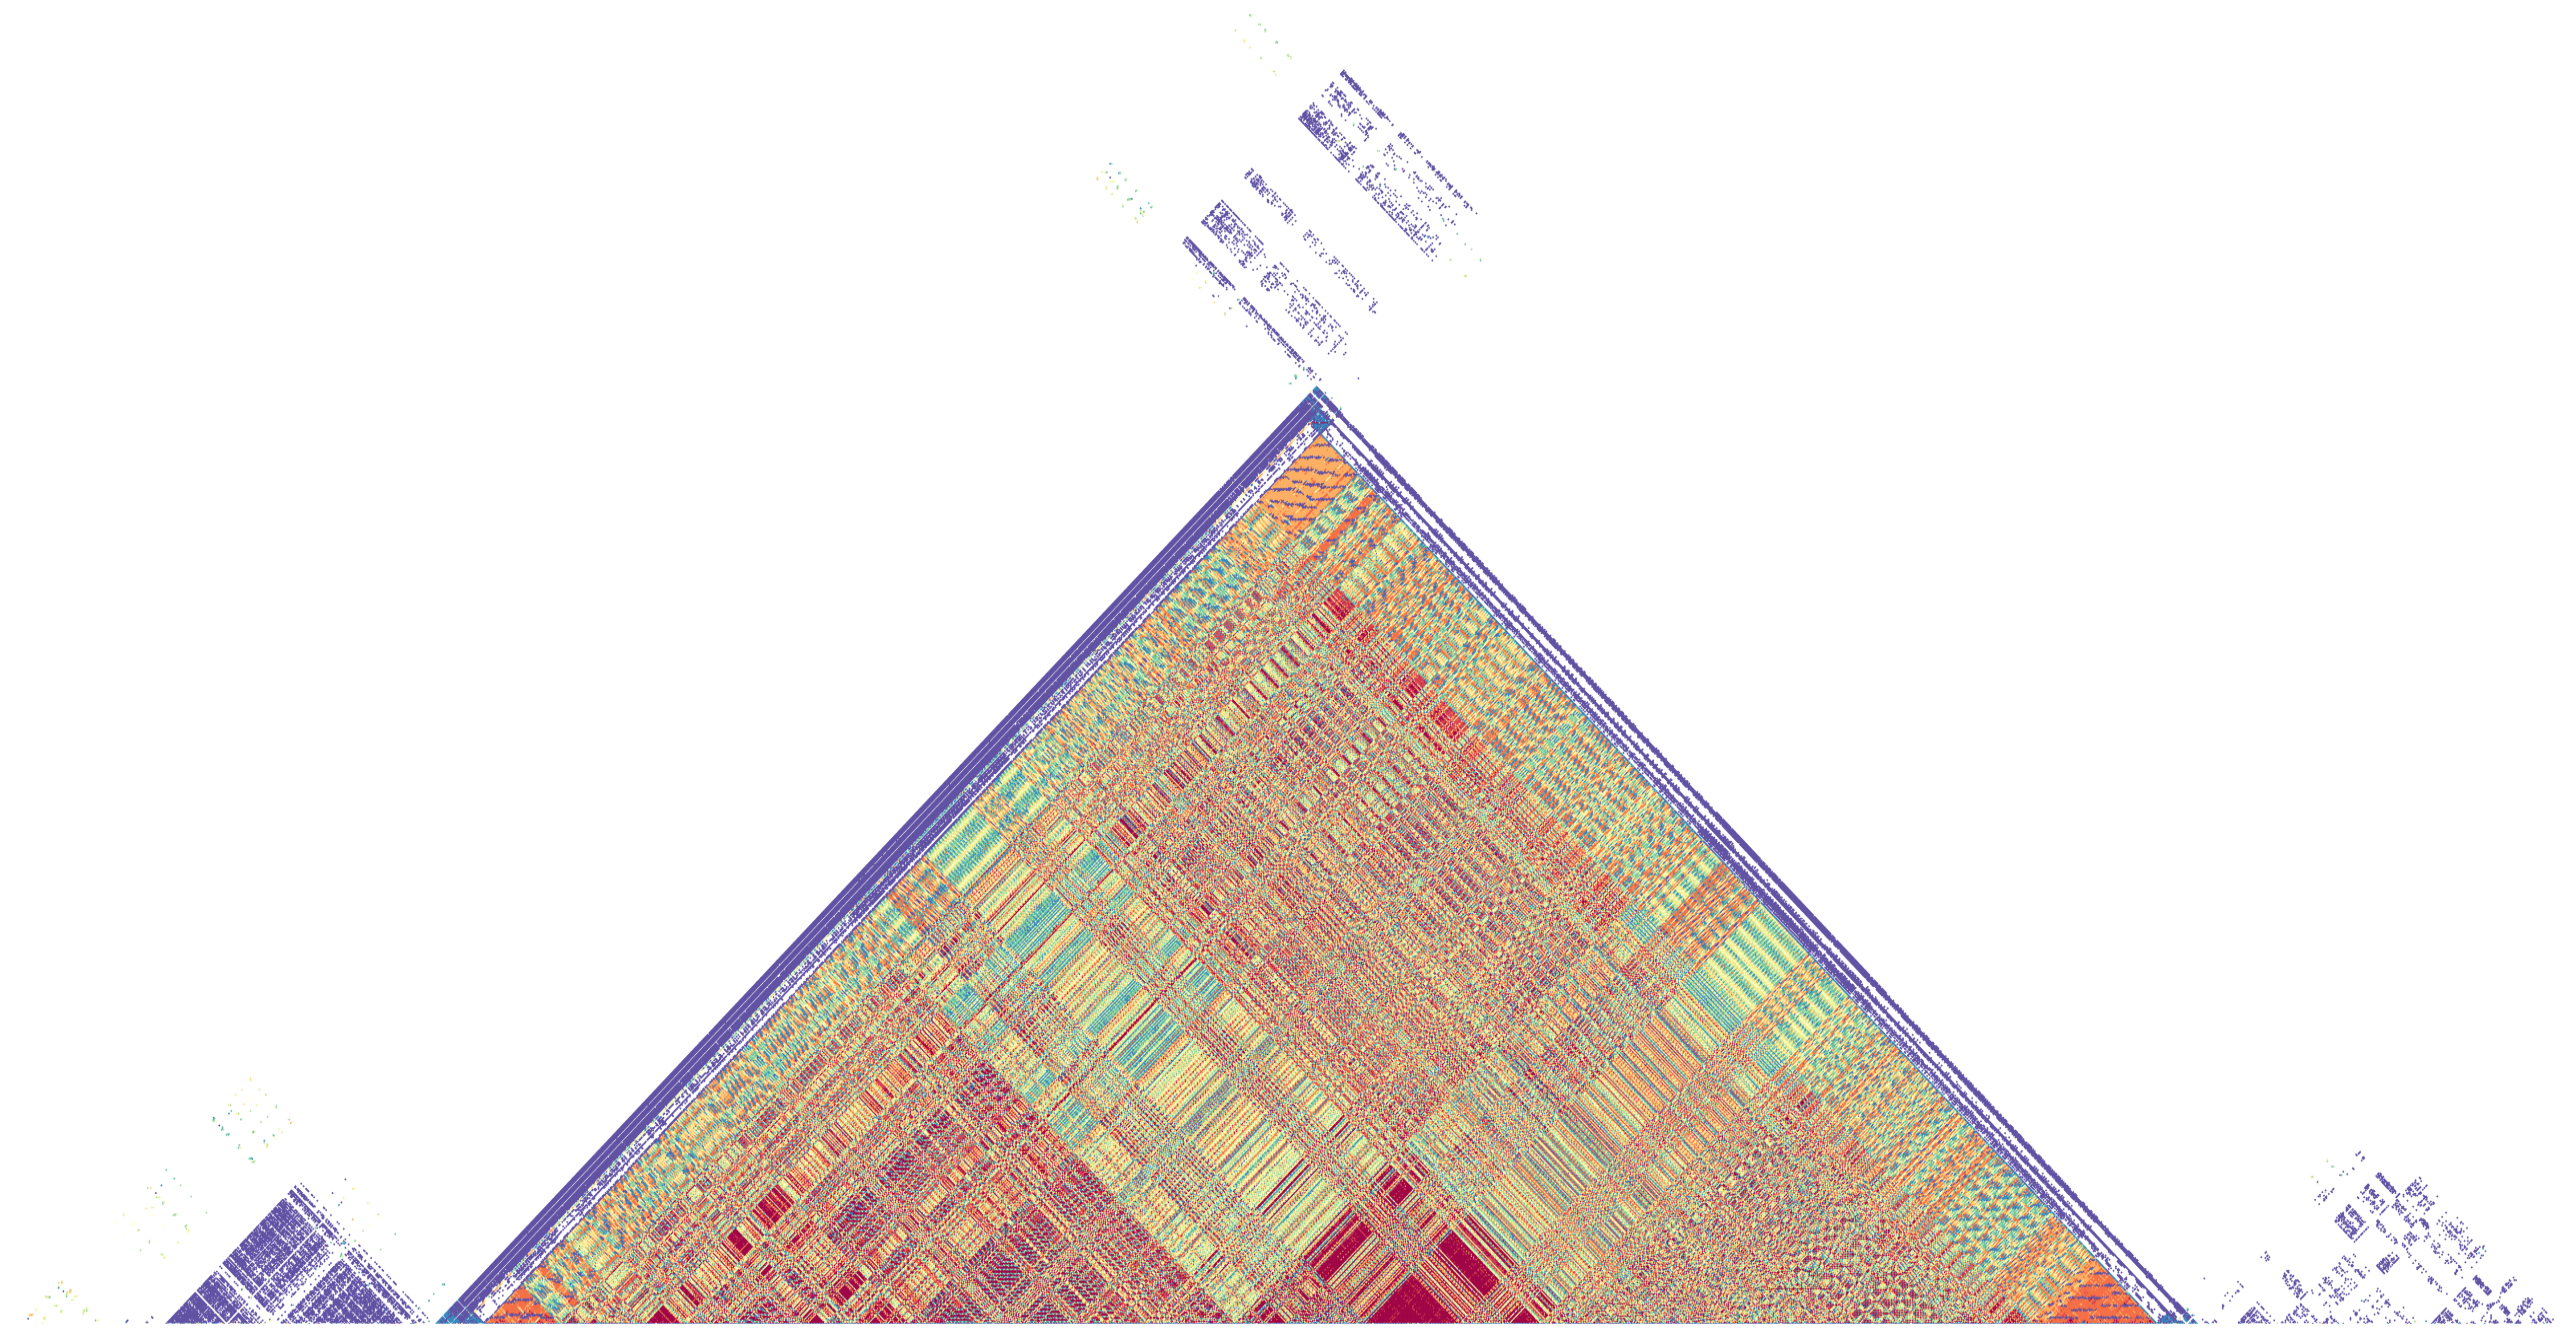
\includegraphics[width=0.5\textwidth,keepaspectratio]{figure1.png}
}
\caption{Output from StainedGlass showing the sequence identity within human
chromosome 8.}
\label{fig:01} 
\end{figure}
%%--------------------------------------------------------------------------%%


To generate pairwise sequence identity dot-plots for StainedGlass the input
sequence is fragmented into windows of a preset size (default 5 kbp) and then
all possible pairwise alignments between the fragments are calculated using
minimap2 (\citealp{Li2018-is}) in an all by all alignment mode. The color used in the
dot-plot is determined by the sequence identity of the alignment which is
calculated as: $$ ID = 100 \biggl( \frac{M}{M+X+I+D} \biggr) $$ where $ID$ is
the percent sequence identity, $M$ the number of matches, $X$ the number of
mismatches, $I$ the number of insertion events, and $D$ the number of deletion
events. When there are multiple alignments between the same two fragments of
sequences all alignments other than the one with the most matches are filtered
out regardless of their sequence identity.

The resulting matrix of percent identity scores can then be visualized using
either static figures, or with HiGlass (\citealp{Kerpedjiev2018-nf}) which allows for interactive data
exploration. The static figures are more appropriate for visualization of 
relatively small regions (30 Mbp or less) at publication quality (Figure
\ref{fig:01}) while the HiGlass visualization is better for data exploration of
whole genome alignments.

The tool is made available using snakemake
(\citealp{Koster2012-fs,Koster2018-ef,Molder2021-xm}) which allows for
reproducible and scalable data analyses. The stability of new changes are
automatically tested with each new change using continuous integration via
github actions. Finally, StainedGlass is
\href{https://snakemake.github.io/snakemake-workflow-catalog?rules=true}{snakemake
standard compliant} so it has automated
\href{https://snakemake.github.io/snakemake-workflow-catalog?usage=mrvollger/StainedGlass}{usage
documentation}.

\section{Usage and examples}
To generate the alignments for StainedGlass you can
execute the workflow as follows. 
\begin{lstlisting} 
	snakemake --use-conda --cores 4 
\end{lstlisting}

To generate the static figures you can add make\_figures to the command.  
\begin{lstlisting} 
	snakemake --use-conda --cores 4 make_figures
\end{lstlisting}

StainedGlass can also be used to make
\href{https://github.com/open2c/cooler}{cooler} files that can be loaded into
HiGlass for whole genome visualizations.
\begin{lstlisting} 
	snakemake --use-conda --cores 4 cooler
\end{lstlisting} 
An example of this interactive browser for the telomere to telomere assembly of CHM13 can be found at 
\href{https://resgen.io/paper-data/T2T/views/MtjcVgrlQmymnHIvdck5-g}{resgen.io}.

\section{Conclusion}

StainedGlass is a visualization tool for large genomic repeats and building on
snakemake makes StainedGlass both reproducible and scalable at the whole genome
level. The output visualizations produced by StainedGlass are publication ready
while also providing an option for interactive data exploration through the use
of HiGlass.

\section*{Acknowledgements} The authors thank T. Brown for help in editing this
manuscript and G. A. Logsdon for aesthetic suggestions.

\section*{Funding}
This work was supported, in part,
by the Intramural Research Program of the National Human Genome Research Institute,
National Institutes of Health (A.M.P.) and grants from the U.S. National Institutes of
Health (NIH grants 5R01HG002385 to E.E.E.; 5U01HG010971 to E.E.E.; and 1U01HG010973 to
E.E.E.). E.E.E. is an investigator of the Howard Hughes Medical Institute.

%\bibliographystyle{achemnat}
%\bibliographystyle{plainnat}
%\bibliographystyle{abbrv}
%\bibliographystyle{plain}

\bibliographystyle{natbib}
\bibliography{StainedGlass}

\end{document}
